\documentclass{article}
\usepackage[T1]{fontenc}
\usepackage{lmodern}
\usepackage{graphicx}
\usepackage{amsmath,amssymb}
\usepackage[a4paper,margin=2cm]{geometry}
\usepackage[absolute,overlay]{textpos}
\setlength{\TPHorizModule}{1mm}
\setlength{\TPVertModule}{1mm}
\usepackage[indonesian]{babel}
\usepackage{hyperref}
\setlength{\emergencystretch}{2em}
% unit: Halaman 36

\begin{document}

% === Halaman 36 (llm) ===

\bullet Enkripsi dilakukan dengan mencari titik potong huruf plainteks dengan huruf kunci:

\vspace{10mm}

\begin{flushright}
\begin{tabular}{lll}
Plainteks & : & \textcolor{red}{terimapesanangulaikambing} \\
Kunci & : & \textcolor{red}{soreangsoreangsoreangsore} \\
Cipherteks & : & \textcolor{red}{LSimMNVWGRRAAMMZRMKNSTWEK} \\
\end{tabular}
\end{flushright}

\vspace{120mm}

Gambar 4.3 Enkripsi huruf $\mathcal{T}$ dengan kunci $\mathcal{S}$

% deskripsi: Tabel Vigenere Square yang menunjukkan pemetaan huruf untuk enkripsi cipher
% bbox normalisasi: [0.0000, 0.2150, 0.7500, 0.9300]
\begin{textblock*}{157.50mm}(0.00mm,63.85mm)
\noindent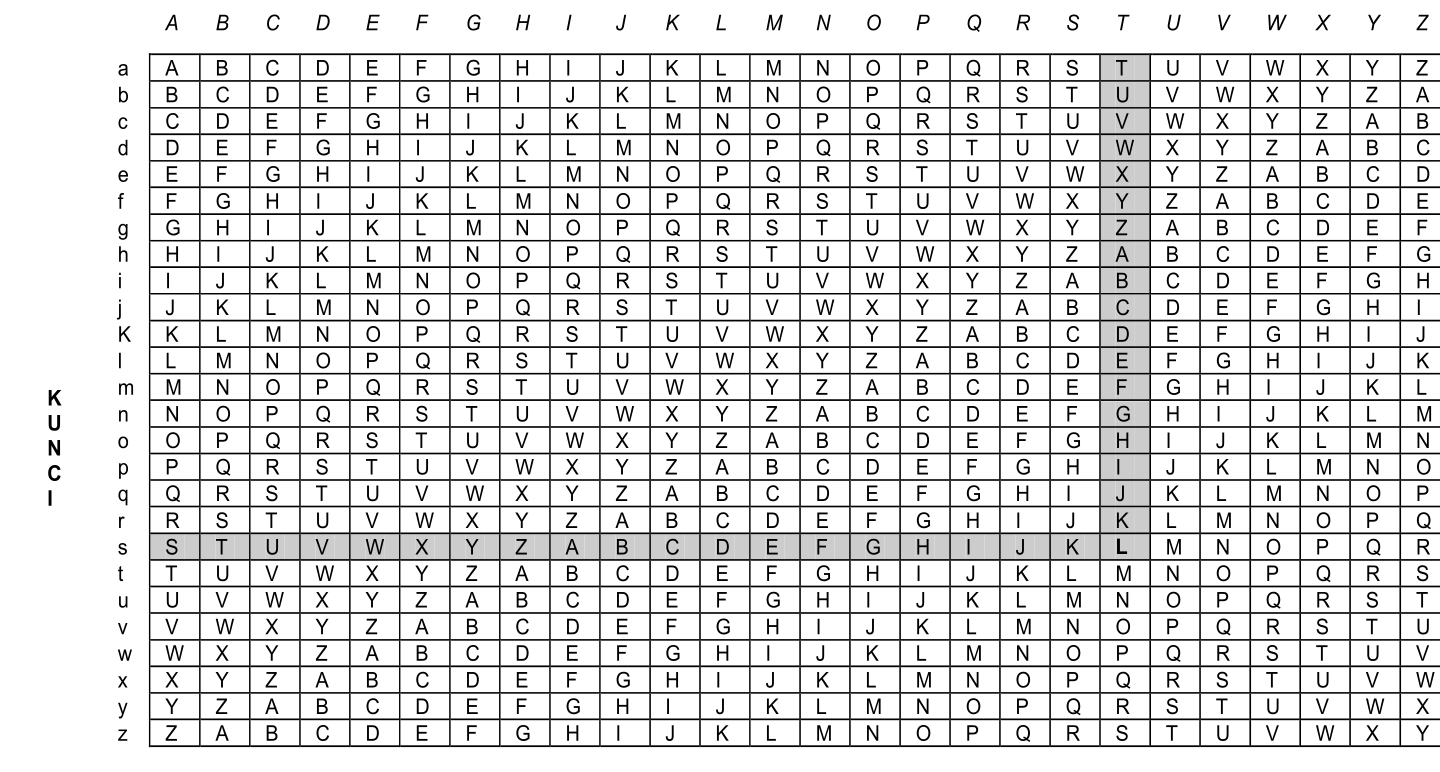
\includegraphics[width=157.50mm,height=212.36mm]{../../images/llm/page_036_img_01.png}%
\end{textblock*}

\end{document}
